% latexmk -pvc -pdf
\documentclass[9pt, a4paper]{article}
\usepackage[margin=0.65in]{geometry}
\usepackage{multicol}
\usepackage{amsmath,amsthm,amsfonts,amssymb}
\usepackage[english]{babel}
\usepackage{blindtext}
\usepackage{caption}
\usepackage{graphicx}
\newenvironment{Figure}
    {\par\medskip\noindent\minipage{\linewidth}}
    {\endminipage\par\medskip}

\title{Measurement of $\beta$-ray spectra}
\author{Ana C. Fabela Hinojosa
\small{School of Physics and Astronomy, Monash University}}
\date{Experiment performed: Tuesday 18\textsuperscript{th} August, 2020,  Submitted: \today}

\begin{document}
\maketitle
\begin{abstract}
Using a thin lens magnetic spectrometer, we measure the momentum spectrum of electrons emitted as $\beta^{-}$ rays from a radioactive source of \textsuperscript{137}Cs. 
The detected momentum of the radiated electrons is defined by the spectrometer's adjustable magnetic lens current and $k$ a proportionality constant dependent on the geometry of the apparatus. The magnetic field of the lens is varied by changing the current passing though the lens coil which has the effect of modifying the trajectories of the electrons, focusing electrons with specific momenta onto the detector allowing us to measure their intensity. By converting the measured momentum to energy we are able to fit our data to a linear model based on the Fermi-Kurie plot. We find that the value of the kinetic energy of the nuclear transition is $T = 0.514 \pm 0.05$ MeV which is in agreement with the accepted value of $T = 0.512$ MeV\cite{SPA}.
\end{abstract}

\section{Introduction}
\begin{multicols}{2}
When Henri Becquerel first observed $\beta-$radiation, he determined that the observed radiated particle satisfied the same mass-to-charge ratio as the electron, discovered in 1897 by J.J Thompson\cite{Wikipedia-particle}. 

Later experimental results showed that $\beta-$rays are detected with a continuous range of kinetic energies up to a maximum value\cite{SMM}. 
The discovery of a continuous distribution of electron kinetic energies rather than a discrete predictable value led Wolfgang Pauli to propose in 1930 that the observed violation of conservation laws must be due emission of a yet unknown particle.

In 1934 Enrico Fermi called this apparently massless and undetectable particle the "neutrino", developing an advanced theory of beta decay. The neutrino was finally experimentally observed 1956.\cite{Nave-beta} 

The process we currently know as $\beta^{-}$ decay describes a neutron in a parent nucleus desintegrating into a proton in a daughter nucleus, an electron and an antineutrino.

In a $\beta^{-}$event, both nuclides (nuclear species) have the same number of nucleons. This means that the daughter nucleus will not experience a substantial change in kinetic energy (recoil) due to the decay event. Leaving most of the desintegration energy available to be carried-off by the leptons as kinetic energy. 

A parent nucleus has a given initial energy $w$. 
The avalilable kinetic energy of the system is equal to the decrease in mass energy due to the creation of the radiated leptons. In relativistic units:
\begin{equation}T = w - 1,
\end{equation}

The observable count of $\beta^{-}$electrons $n$ as a function of energy is described by the Kurie--Fermi Theory of $\beta^{-}$decay.

\section{Background Theory}

In this experiment we measure the momentum spectrum of emitted $\beta-$rays from a radioactive source of \textsuperscript{137}Cs into an excited state of \textsuperscript{137}Ba. This transition occurs with a probability of $94.6\%$ at a maximum energy value $T = 0.512$ MeV.\cite{SPA}.

A set of electrons with a specific momentum range is focused onto the spectrometer detector, while electrons outside this range undergo chromatic aberration. 

The use of coordinates of momentum instead of energy in $\beta-$ray spectroscopy is partly due to the fact that it is the momentum of the focused electrons that is rigorously proportional to the axially symmetric magnetic field.\cite{QH, Siegbahn} 
In our experimental setup, the magnetic field is proportional to the adjustable current $I_{lens}$ going through the lens coils.
The definition for the momentum of emitted electrons is:
\begin{equation}p = e \rho B,
\end{equation} 
where $B$ is the magnetic field strength, $e$ is the electron charge, $\rho$ is the gyroradius of the electrons due to B.

The magnetic rigidity $P$ is a measure of the momentum of electrons\cite{Wikipedia-Rigidity}:
\begin{equation}P = B \rho,
\end{equation}

From this relation and the above definition of the momentum of electrons, we write:
\begin{equation}p = kI_{lens},
\end{equation}
k is a constant determined by the geometry of the spectrometer alone\cite{QH}.

\subsection{K-peak Calibration}

To calibrate the observed momentum distribution we use electrons emitted with a characteristic well-defined kinetic energy\cite{SPA}.
These electrons are named conversion electrons.
In this experiment we study the most probable energy transition from \textsuperscript{137}Cs to \textsuperscript{137}Ba. in this transition \textsuperscript{137}Ba is in an excited state. 
One way for the daughter atom to lose energy is by transferring the excess energy directly to an orbital electron\cite{SPA}.

The orbital will most likely be the K-shell since it is the lowest energy orbital. A higher energy group event is much rarer (probability of $6\%$), therefore little error is made  by assuming that the peak is due to the K line only.\cite{SPA}.

The constant $k$ in (3) is determined by calibrating the observed spectrum to the well-known K-conversion peak with kinetic energy $T_k = 624.21$ keV.
In relativistic units, the calibration calculation is as follows:
we write equation (1) in terms of the momentum $p_k$
\begin{equation}T_k = \sqrt{{p_{k}}^{2} + 1} -1,
\end{equation}
\begin{equation} \therefore p_k = \sqrt{({T_{k} + 1)}^{2} - 1 },
\end{equation}
from equation (4)
\begin{equation} k I_k = \sqrt{({T_{k} + 1)}^{2} - 1 },
\end{equation}
\begin{equation} \therefore k = \frac{\sqrt{({T_{k} + 1)}^{2} - 1 }}{I_k},
\end{equation}is the proportionality constant we are after.

\subsection{Kurie--Fermi theory}

The standard method for determining end-points of $beta-$ray groups and for examining the degree of forbidden-ness of the transitions\cite{SPA} is known as the Kurie plot. The observed maximum value in the Kurie--Fermi plot represents the count of electrons that take the maximum possible kinetic energy whilst the antineutrinos carry close to zero kinetic energy from the transition.

The Kurie--Fermi plot may be written as: 
\begin{equation} n(p) = K_1 F(Z, w) p^2(w_0 - w^2) S_n(w),
\end{equation}
where $K_1$ is an arbitrary constant, $p$ is the electron's momentum, $F(Z, w)$ is the Fermi function (which accounts for coulomb attraction between the electron and the daughter nuclleus). $Z$ is the charge of the daughter nucleus, $w_0$ is the decay energy, and $w$ is the total transition energy and $S_n(w)$ is known as the shape factor. 

In our analysis we use a modified Fermi function: 
$G = \frac{p F(Z=55, w)}{w}$. We find The value of this function using an interpolation method based on a data set provided in the aditional resources of the experimental script.

In order to use this relation to obtain the transition energy, we are told linearise the Kurie plot. 
Written in terms of the interpolated fermi function, we write the linear kurie plot as:
\begin{equation} \sqrt{\frac{n(p)}{p^2 w G S_n(w)}}= K_2 (w_0 - w)^2,
\end{equation}

The shape factor alters the shape of the spectrum depending on the level of “forbiddeness” of a transition. It is determined by the amount of orbital angular momentum, $L$, carried away by the electron-neutrino pair, as well as their linear momenta)\cite{NERS312}.

We obtain an expression for the shape factor from Siegbahn, reference\cite{Siegbahn}:
\begin{equation} S_n = w^2 - 1 + (w_n - w)^2,
\end{equation} 

The shape factor increases the precision of the result as the order icreases. The zeroth order linear Kurie plot is found by calculating
\begin{equation} \sqrt{\frac{n(p)}{p^2 w G}}= K_2 (w_0 - w)^2,
\end{equation}
where the transition is allowed: $S_0(w) = 1.$

We proceed to find the zeroth order energy transition $w_0$ 
\begin{equation} w_0 = \frac{c}{-K_2},
\end{equation}
After we have obtained $w_0$ we can iteratively repeat the previous analysis. 
From this we obtain higher order $w_n$ and $S_n$ values. We use the results from the iteration to find a convergent value for $T$ the transition energy.

\section{Method}

Our experimental apparatus is a thin magnetic-lens spectrometer. 
The operation of $\beta$ spectrometers depends on the behaviour of electrons subject to magnetic fields. 

The spectrometer is aligned parallel to the horizontal component of the Earth's magnetic field, Then the horizontal component of the field does not affect the electron paths. The vertical component is nullified by an adjustable bias coil current from a pair of Helmholtz coils.

The magnetic field of the spectrometer lens is varied by changing the current passing though the lens coils.
Modifying a cone of electron trajectories diverging from the source along the spectrometer's axis, causing them to spiral around the axis of the instrument towards detector\cite{SPA}. 

\subsection{Constant time vs constant counts}

The counting controls of the experimental apparatus can be defined by the user.
For constant time, the best estimation for the uncertainty in the number of counts $n$ is $\sqrt{n}$\cite{SPA} due to the poissonian nature of radioactive decay. 
The fractional uncertainty in counts is $\frac{\sqrt{n}}{n} = \frac{1}{\sqrt{n}}$
Fractional uncertainty is a preserved quantity. Therefore the uncertainty in time
is :$ \Delta t = \frac{t}{\sqrt{n}}$ 

From this result we note that with both methods we are able to pre-determine the fractional uncertainty for a data point. 
But an obvious constraint from choosing the constant counts method is that the alloted time for the experiments is not as easily monitored as with constant time. 
Given the possible time constraint. The counting controls are set to constant time. 
The interval used to count events isdefined by trying to mantain the uncertainty in the count as less than 5 percent.

\begin{equation}\frac{t}{\sqrt{n}} \leq \frac{1}{20},
\end{equation}
\begin{equation}\therefore n \leq 400,
\end{equation}

From an earlier attempt at the experimental data acqusition we learned that the maximum time interval $t = 600s$ yielded  $n \approx 2000$ counts. A simple calculation comparing the count ratios yields the time interval $t = 360s$ as the upper bound for our constant time interval.

\subsection{Background radiation}

After we obtain the raw spectrum $n_{\mathrm raw}$ as a function of the lens current. The first processing step is to correct our data from the background radiation count.
The 4 measurements of the background radiation counts are added, averaged and the average is subtracted from the raw count.

\subsection{Resolution}

In a magnetic spectrometer with fixed geometry and variable $B$ the resolution 
\begin{equation}R = \frac{\Delta(B \rho)}{B \rho},
\end{equation}
is constant (in this experiment $R = (2-3\%)$). 
Where $\Delta(B \rho)$ is a measure of the accepted momentum band ($\Delta p$). 
When plotting the momentum distribution it is necessary to divide the number of counts n(p) at each current setting by the corresponding current in order to get the correct form of the spectrum\cite{Siegbahn}.
\begin{equation} n(I) = \frac{n_{\mathrm net}}{I_{\mathrm lens}},
\end{equation}

\subsection{Experimental procedure}

Firstly, Decide what range and increments of lens current are adequate to resolve the momentum spectrum.
Then, using the experimental control interface:
\begin{enumerate}
\item Calibrate the magnetic field probe.
    Coordinates of the probe must be set to: $(400,190)$
\item Null Earth's magnetic field:
    Disable the lens current.
    Enable the bias coil current and increase this current until all displayed field values are as close to zero as possible. 
    Note: (the x-component of the field will remain large compared to the other components.)
\item Set counting controls to either constant time or constant counts.
    Specify time interval or expected counts.
\item Background rate count:
    Close the source shutter.
    With the lens current disabled, proceed to run the experiment and count the background radiation (repeat this step 4 times).
\end{enumerate}
After these steps are finalised we can start acquiring $\beta^{-}$ radiation data from our source of \textsuperscript{137}Cs.
\subsection{Data acquisition algorithm}
\begin{enumerate}
\item Enable the lens coil current.    
\item Set the shutter status to open.
\item Run the experiment.
\item Increase the lens coil current.
Repeat steps (3-4) until reaching the maximum value of the coil current range.
\end{enumerate}

\section{Results}

The experimental parameters used are as follows:
The lens current range is set from $0$A to $3.6$A
Increments of $0.1A$ are chosen. 
To minimise earth's magnetic field we set the bias coil current to $I = 0.7167 \pm 0.0005$
Counting controls were set to constant time: The intervals $t = 360$s.

\subsection{The momentum spectrum}
We calibrate the measured spectrum by using the conversion peak energy $T_k$. 
Using equation $(10)$ we proceed to find the constant of proportionality in equation $(5)$.

Table I. K-peak parameters and uncertainties.
\begin{center}
\begin{tabular}{ c c c c }
\hline
\hline
\phantom & $I_k$ & \phantom & 1.89 \\ 
\phantom & $u(I_k)$ & \phantom & 0.05  \\
\phantom & $k$ & \phantom & 1.05  \\
\phantom & $u(k)$ & \phantom & 0.03 \\
\hline
\hline
\end{tabular}
\end{center}

Table II. Corrected count, momentum, energy data and uncertainties.
To be used in linear Kurie Plot, We compute the relativistic energy value from the momentum $w = \sqrt{p^2 + 1}$.
\begin{tabular}{ c c c c c c }
\hline
\hline
n & u(n) & p [mc] & u(p) [mc] & $w [mc^2]$ & $u(w) [mc^2]$ \\
\hline
1612 &  20 & 0.73 & 0.02 & 1.24 & 0.02 \\
1441 &  20 & 0.83 & 0.02 & 1.30 & 0.02 \\
1318 &  18 & 0.94 & 0.03 & 1.37 & 0.02 \\
1291 &  16 & 1.04 & 0.03 & 1.44 & 0.03 \\
1040 &  15 & 1.15 & 0.03 & 1.52 & 0.03 \\
798 &  14 & 1.25 & 0.03 & 1.60 & 0.03 \\
589 &  13 & 1.36 & 0.04 & 1.68 & 0.04 \\
356 &  12 & 1.46 & 0.04 & 1.77 & 0.04 \\
190 &  11 & 1.57 & 0.04 & 1.86 & 0.04 \\
62 &  10 & 1.67 & 0.04 & 1.95 & 0.04 \\
\hline
\hline
\end{tabular}

\begin{Figure}
 \centering
 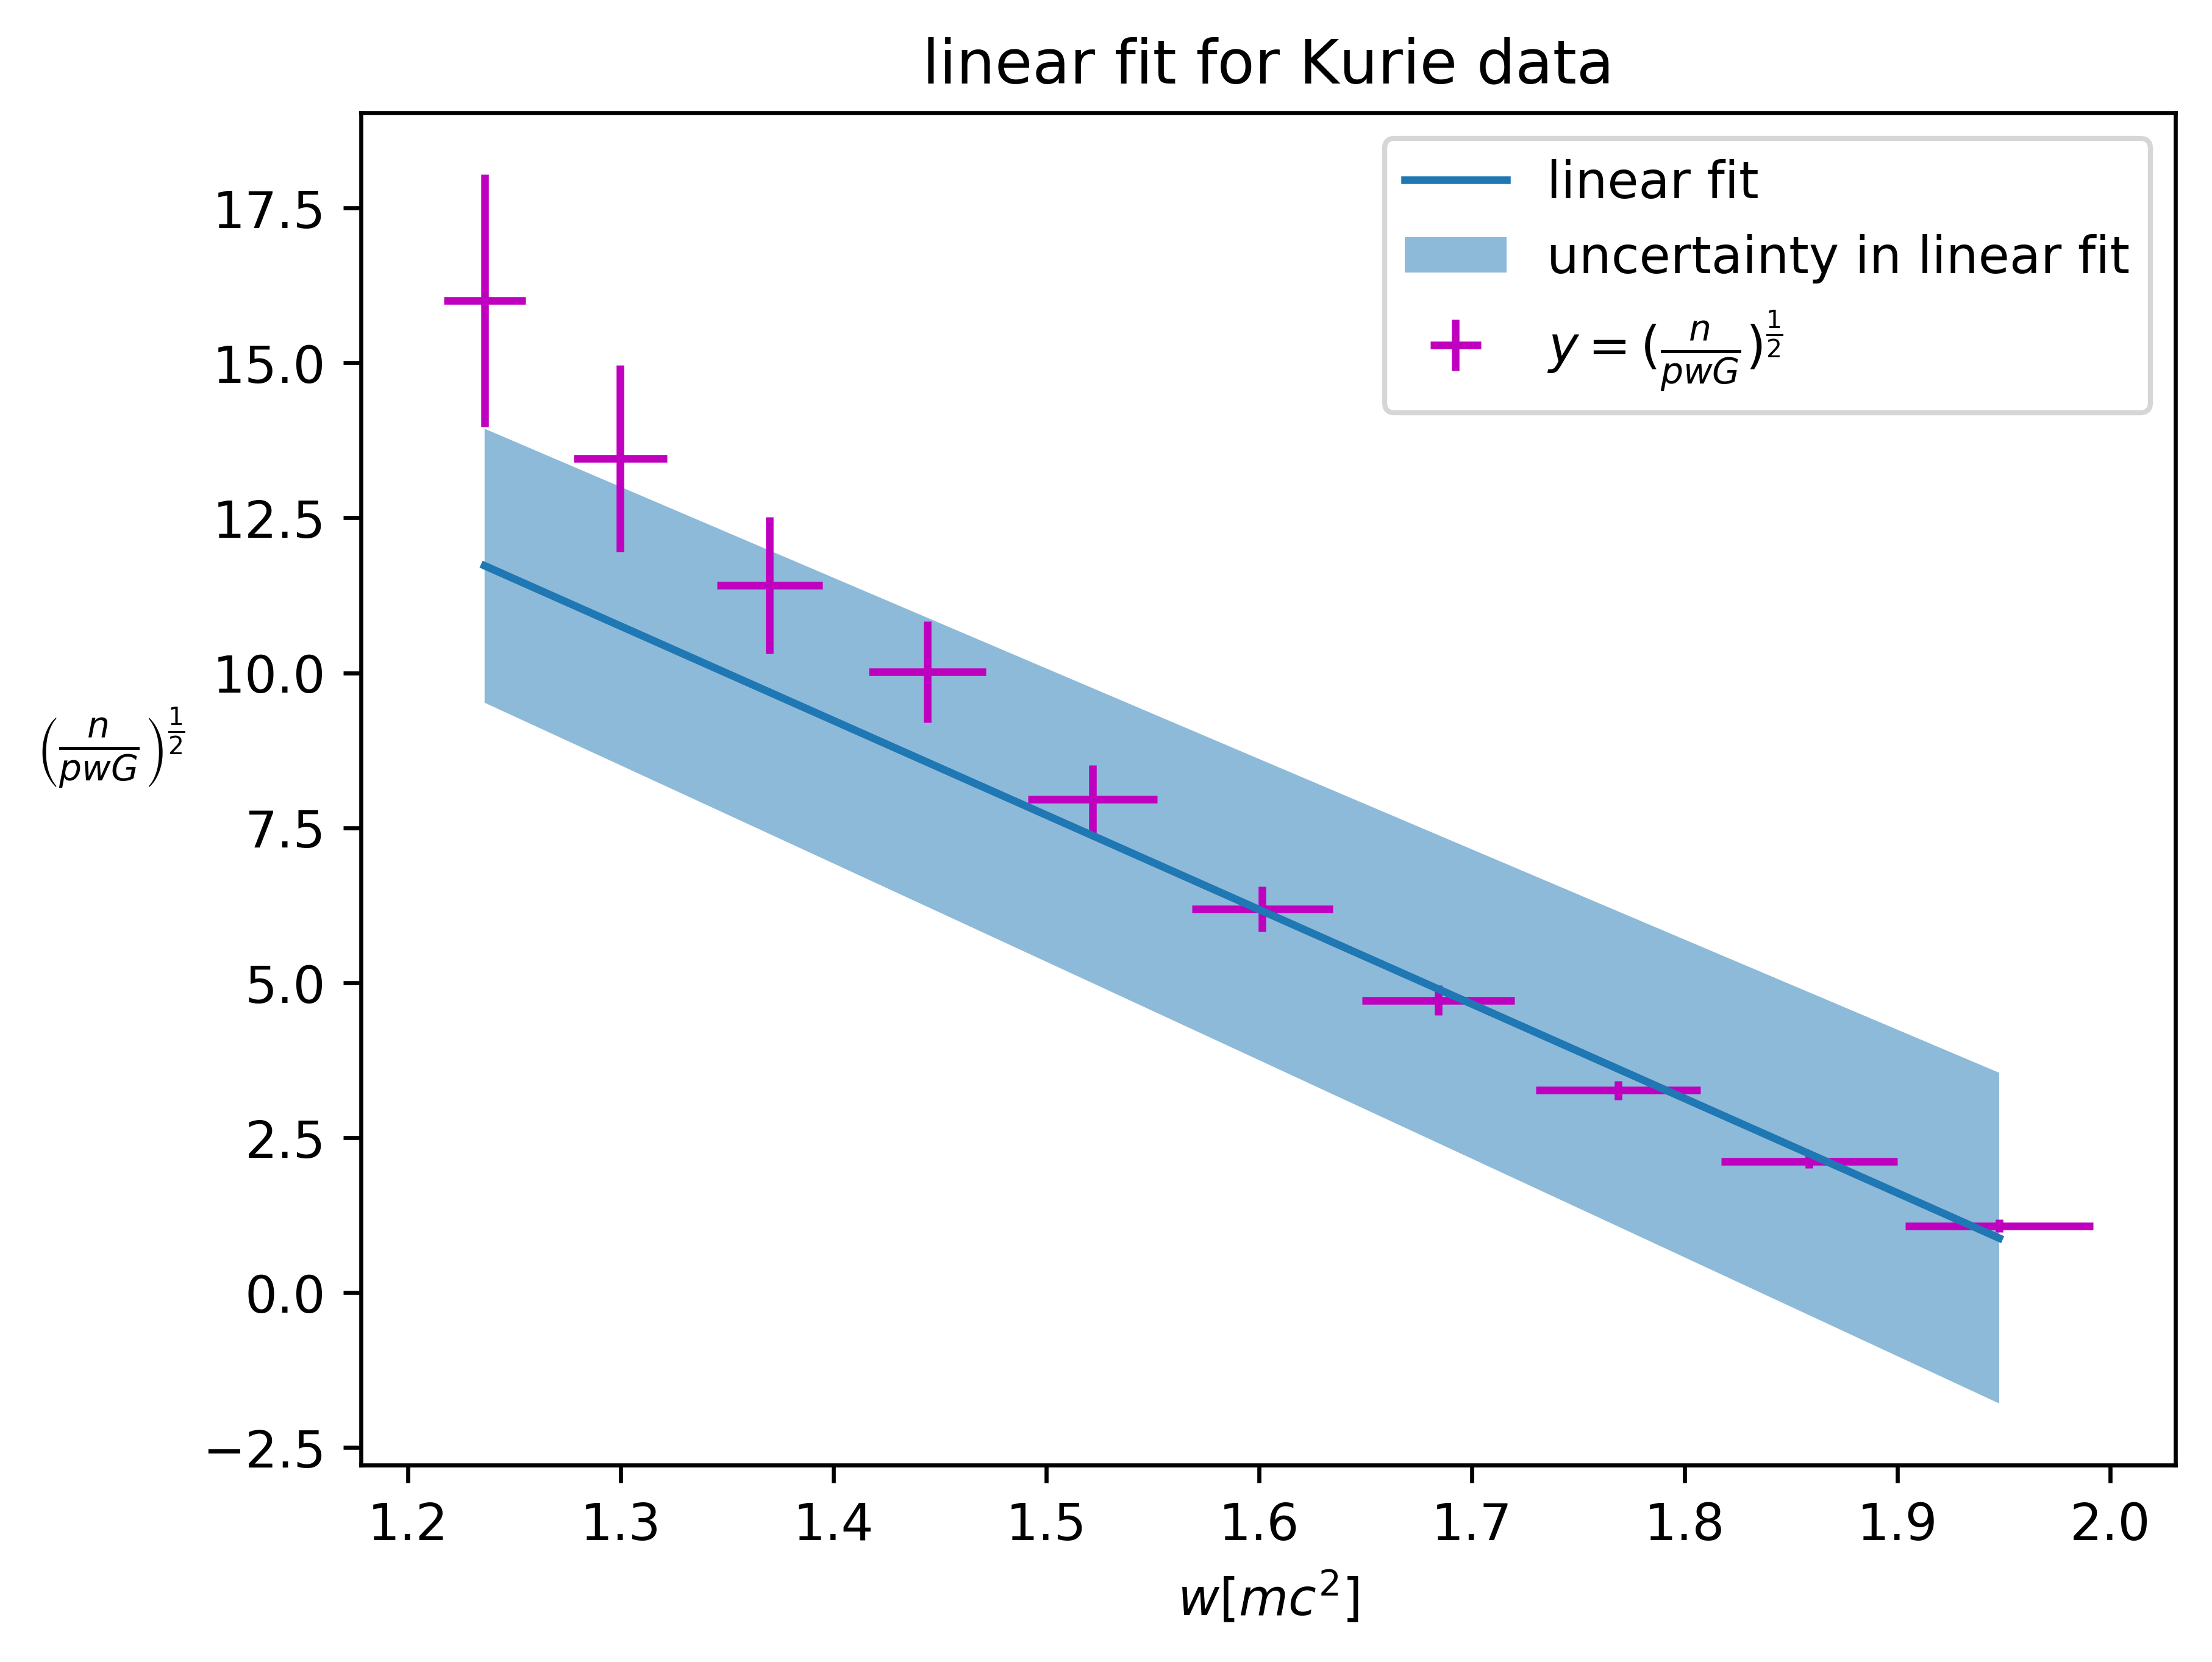
\includegraphics[width=\linewidth]{Kurie_linear_data_plot.png}
 \captionof{figure}{Linear fit was obtained using the curve\_fit optimisation algorithm from the Scipy library.}
\end{Figure}

\begin{Figure}
 \centering
 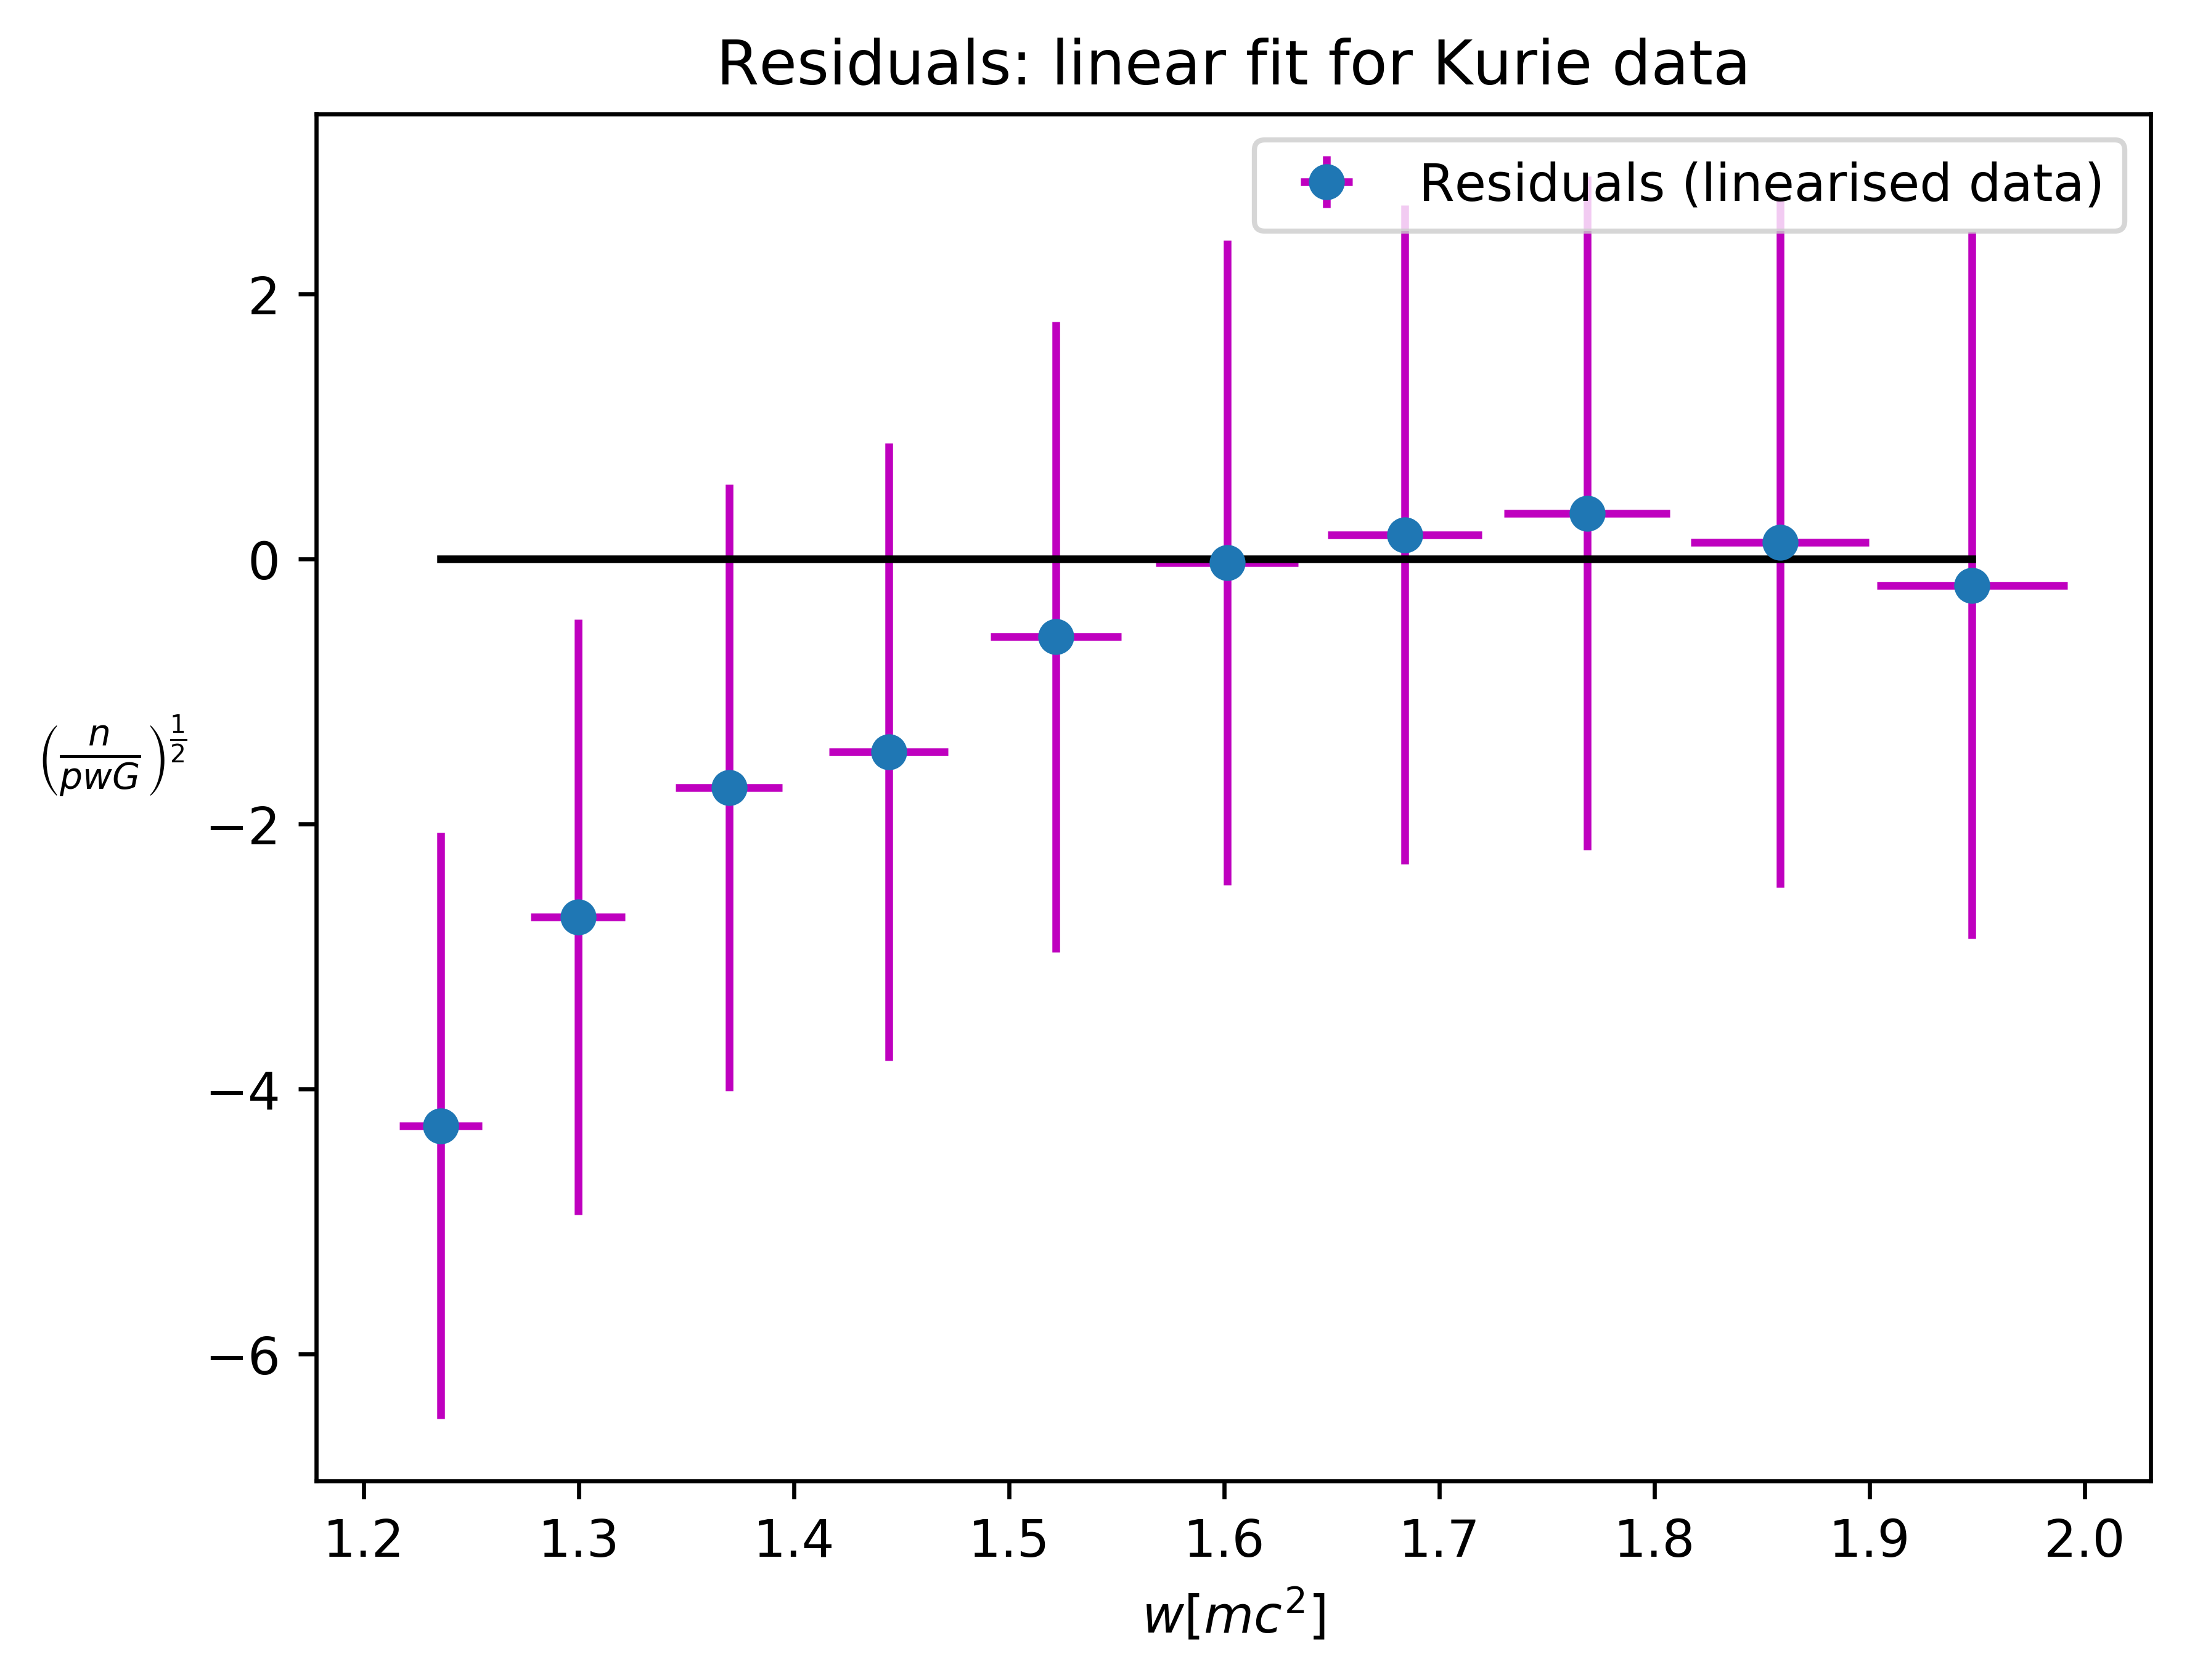
\includegraphics[width=\linewidth]{linear_residuals_Kurie_linear_data.png}
 \captionof{figure}{Linear fit residuals for optimised Kurie plot data.}
\end{Figure}

In equation $(14)$ we defined a zeroth order fit for the Kurie Plot. $S_0 = 1$ 
Using an optimised fitting algorithm we determine the optimal parameters for this linear fit.
From these parameters and equation $(15)$ we find $w_0 = 1.03 \pm 0.04$ MeV.

Using $w_0$ we calculate higher order approximations of shape factor $S_n$ which in turn increases the order and accuracy of $w_n$.
Finally we find that $T = 0.514 \pm 0.05$ MeV. This value is $\sigma = 0.04$ away from true result $T = 0.512$ MeV.

\section{Discussion}

The dominant problem in our analysis is the process by which we obtained the value of the proportionality constant $k$. It unlikely that we have found the true value $I_k$. The value of $I_k$ was simply set to the corresponding current measured for the apparent conversion peak. 
Since there are only 2 data points visible in our conversion peak a better method would have been to create a lorentzian fit for the data. Unfortunately we were not able to write code and perform this fit adequately so the naive method remained.

Our experimental execution and the theoretical framework of $beta$-decay we use in this report ignores the mass of the neutrino. We hypothesize that the fact that the electrons are emitted with specific momentum ranges is likely closely related to the varying mass of emitted neutrinos. 

There are three neutrino flavor states and three discrete neutrino masses with different values (they do not correspond uniquely to the three flavors). A neutrino created with a specific flavor has an associated specific quantum superposition of all three mass states\cite{Wikipedia-Neutrino}. 

It is presently known that neutrinos oscillate between different flavors during flight. This oscillation occurs because the three mass state components of the produced flavor travel at different speeds.
This means that relative phase shifts between their wave packets develop. 
Their interaction with the detectors determines how their wave packets combine to produce a varying superposition of three flavors\cite{Wikipedia-Neutrino}. 

\section{Conclusion}

Using a magnetic spectrometer we measure the energy spectrum of electrons emitted as $\beta$ radiation from a \textsuperscript{137}Cs source. Our investigation focuses in determining the relationships between the spectrometer's lens current, electrons' momenta and their energy. We find that the value of the kinetic energy of the nuclear transition is $T = 0.514 \pm 0.05$ MeV which is in agreement with the accepted value of $T = 0.512$ MeV.


\end{multicols}
\bibliography{mybib}
\bibliographystyle{unsrt}
\end{document}